\documentclass[10pt,twocolumn,letterpaper]{article}
\usepackage[review]{cvpr}
\usepackage{graphicx,amsmath,amssymb,booktabs,microtype,multirow}
\definecolor{cvprblue}{rgb}{0.10,0.43,0.58}
\definecolor{oursteal}{HTML}{008C88}
\usepackage[pagebackref,breaklinks,colorlinks,allcolors=cvprblue]{hyperref}
\def\confName{CVPR}\def\confYear{2027}
\newcommand{\R}{\mathbb{R}}
\newcommand{\ours}{\textsc{PositionTwin}}
\title{Position-Driven Deformable Twins:\\Separating Material Response from Interaction Conditions}
\author{Anonymous submission}
\begin{document}
\twocolumn[{
\renewcommand{\twocolumn}[1][]{#1}
\maketitle
\begin{center}
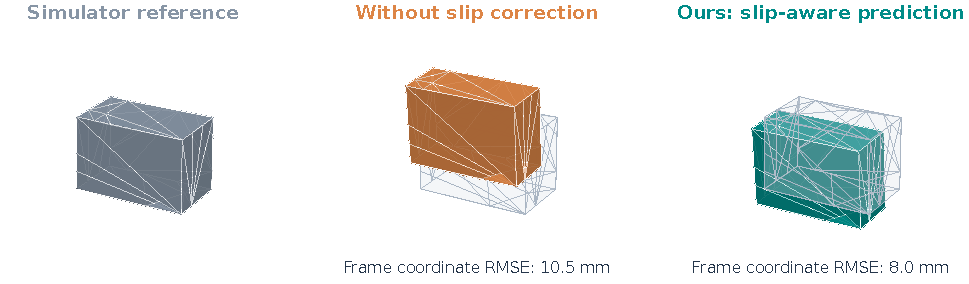
\includegraphics[width=.98\textwidth]{figures/teaser.pdf}
\captionof{figure}{\textbf{Predicting what happens after the observation ends.} SoftVTBench forecast at the same time and in the same world coordinates. Gray reference points reveal displacement from the target. Modeling controller-relative slip improves the object's predicted placement. This is the largest episode-level improvement among 40 fresh episodes, shown at 75\% of its forecast interval; aggregate results include all 40. Surfaces connect the initial node convex hull for visualization; vertex positions are the unaltered saved states.}
\label{fig:teaser}
\end{center}
}]
\begin{abstract}
A deformable digital twin must respond to a changed interaction, not only reproduce observed motion. We study position-driven prediction with a representation that distinguishes material response, tool-relative attachments, and world-space loading and support. Initial geometry and a short sequence of observed positions define a scene-specific inverse problem; future tool positions drive the resulting twin without requiring a measured force trajectory. We instantiate this formulation with an analytic mechanics and slip-release adapter for SoftVTBench, and a frozen neural constitutive adapter for real PhysTwin captures. On 40 fresh SoftVTBench episodes, slip-aware prediction reduces coordinate error from 18.93 to 17.86\,mm, improving 36 episodes and completing all 1,998 forecast frames. On two real cross-interaction pairs passing an initial-geometry compatibility test, the neural adapter reduces tracking error from 44.63 to 39.16\,mm relative to an adapted frozen PhysTwin baseline. We also report the complete eight-sequence reconstruction benchmark, where native PhysTwin remains stronger. Separate geometry, deformation and shared-appearance measurements reveal when interaction modeling helps, and when visually plausible predictions still lack accurate physical response.
\end{abstract}

\section{Introduction}
Consider a robot lifting a soft object. The visible motion combines the commanded movement of the gripper, deformation of the object, and motion at the attachment. If the object slips, a predictor that interprets all observed motion as elastic deformation can reproduce a short prefix yet place the object incorrectly after release. A second camera may improve the reconstructed shape, but it does not by itself specify the interaction law that determines the next motion.

We address this distinction through a position-driven digital twin. The twin receives observed positions and known tool motion, estimates effective material and interaction parameters, and predicts a response to subsequent tool commands. Material properties move with the object; attachments are defined relative to tools; gravity and environmental support act in world coordinates. This separation makes the source of each prediction explicit and provides a practical way to change an interaction while retaining the fitted material.

Our objective is predictive behavior under changed commands. Rendering and physical prediction are evaluated separately: a Gaussian appearance model can remain fixed while the predicted mechanics changes. We consolidate two completed external-dataset studies around this formulation, with the implementation used for each dataset stated explicitly. This produces a focused evaluation of position-driven mechanics rather than a claim that one end-to-end video network solves all aspects of digital-twin construction.

\begin{figure*}[t]
\centering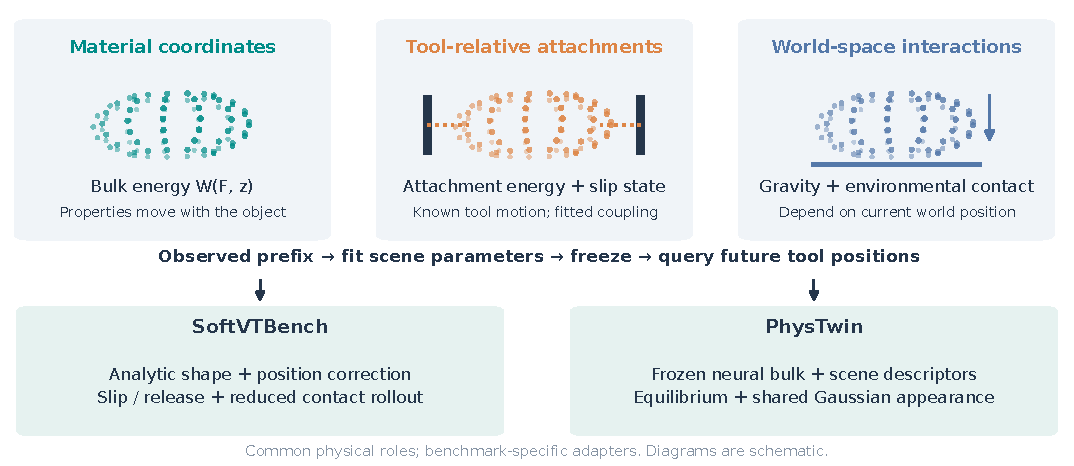
\includegraphics[width=\textwidth]{figures/method.pdf}
\caption{\textbf{Position-driven prediction with explicit physical roles.} Observations fit a scene, while future tool positions query it. Material, attachments and world-space interactions remain distinct. The two benchmark adapters share this interface but use different constitutive and rollout implementations; their results are not attributed to one shared checkpoint. Appearance evaluation is available on PhysTwin.}
\label{fig:method}
\end{figure*}

\paragraph{Contributions.}
First, we formulate a common position-conditioned representation with separate material, relational and environmental terms. Second, we evaluate two concrete instantiations: a slip-aware reduced interaction model for manipulation episodes, and a frozen constitutive decoder adapted to real reconstructed geometry. Third, we provide an evaluation that distinguishes ordinary sequence continuation, frozen cross-interaction transfer, internal deformation, and image agreement. The strongest evidence is a complete prospective episode improvement on SoftVTBench and a small positive real-transfer pilot. We retain the full real-data comparison rather than equating transfer gains with overall benchmark leadership.

\section{Related Work}
\paragraph{Visual assets with physical dynamics.}
Gaussian splatting represents appearance through explicit spatial primitives~\cite{kerbl2023gaussians}. PhysGaussian couples these primitives to continuum simulation, allowing supplied materials and boundary conditions to drive motion~\cite{xie2024physgaussian}. Spring-Gaus reconstructs elastic objects using spring-mass dynamics and Gaussian rendering~\cite{zhong2024springgaus}. PhysTwin combines sparse RGB-D observations, geometry completion, spring-mass inverse modeling and appearance optimization to produce interactive deformable twins~\cite{jiang2025phystwin}. These methods demonstrate that physical simulation and rendering can be integrated effectively. Our comparison asks how fitted representations behave when positional interactions change, and separates that question from the quality of appearance reconstruction.

\paragraph{Inverse physics and reusable material laws.}
PAC-NeRF combines radiance fields with differentiable continuum simulation for system identification~\cite{li2023pacnerf}. NCLaw learns constitutive response within known governing equations, supporting transfer across geometry and boundary conditions~\cite{ma2023nclaw}. UniPhy pretrains latent-conditioned constitutive networks and subsequently fits a material latent to observed trajectories~\cite{mittal2025uniphy}. We follow the established principle of separating a reusable material prior from scene-specific adaptation. Our neural adapter uses a scalar energy, obtains stresses by differentiation, and combines the bulk law with explicit tool attachments and environmental terms. The analytic adapter tests the same separation without a learned bulk decoder.

\paragraph{Reconstruction and physical plausibility.}
PhysDreamer uses generative video priors to obtain plausible interaction responses~\cite{zhang2024physdreamer}. PIDG associates Gaussian particles with time-evolving constitutive fields and uses momentum residuals and optical-flow supervision for dynamic reconstruction~\cite{hong2026pidg}. These are relevant approaches to motion and physical structure, but their reported tasks and inputs differ from a frozen twin queried with new tool trajectories. We discuss them as related work; we do not report an unimplemented numerical comparison against PIDG or reinterpret a reconstruction score as an action-prediction score.

\paragraph{Evaluation resources.}
SoftVTBench supplies simulated deformable manipulation episodes with synchronized observations and evaluator-side finite-element states~\cite{jing2026softvt}. Its native benchmark evaluates closed-loop manipulation and deformation-aware success. We instead define a privileged sparse-position forecasting protocol on its released episodes. PhysTwin provides real interaction captures and reconstructed tracking annotations~\cite{jiang2025phystwin}. Together they expose complementary errors: the simulator provides known positions, whereas real captures include reconstruction uncertainty, occlusion and imperfect geometry. Their metrics are reported separately.

\section{Position-Driven Scene Representation}
\subsection{What is observed and what is queried?}
Let $X_i\in\R^3$ be a reference material point and $x_i(t)$ its world-space position. Initial geometry defines a tetrahedral discretization and a fixed interpolation operator $A$ from mechanical nodes to observed points. At times $t\leq T_o$, the input contains sparse positions $y_t$, visibility masks $V_t$, and tool poses. At query time, the model receives future tool positions or poses $a_t$, together with the scene's fixed environmental geometry. The desired output is the node trajectory $\hat x_t$ and its interpolated observable geometry.

No future object positions, measured force trajectory, or ground-truth material coefficients enter the predictor. Geometry and correspondences are supplied by the benchmark adapter. We therefore study a downstream inverse-mechanics problem rather than image-only reconstruction. The first observed configuration is used as an effective rest shape; this practical approximation can absorb unknown prestress into fitted parameters.

\subsection{Material, attachment and environmental terms}
We define the scene potential as
\begin{align}
\Pi(x;z,a)={}&\sum_e V_e W(F_e;z_m(X_e))\nonumber\\
&+\frac12\sum_{b,i}\alpha_b(t)K_b w_{bi}\|x_i-T_{bi}(a_t)\|^2\nonumber\\
&-\sum_i m_i g^\top x_i+\Pi_{\mathrm{env}}(x;z_e),\label{eq:potential}
\end{align}
where $F_e$ is the deformation gradient, $V_e$ is reference volume, $z_m$ describes material response, and $T_{bi}$ is a tool-conditioned target for node $i$. Attachment activity $\alpha_b$ follows the input gripper state or the adapter's declared release rule. The normalized footprint $w_{bi}$ localizes a tool's influence without changing its total stiffness $K_b$.

The coordinate systems encode distinct physical roles. A stiffness feature $z_m(X)$ remains attached to material even after rigid motion. The attachment residual is relative to a moving tool. Gravity and floor contact depend on the current world position. Thus changing a camera does not change the mechanics, and changing a tool pose does not require redefining the material field.

For arbitrary reconstructed objects, we form tetrahedra from the initial cloud. Tetrahedra whose center or edge-midpoint probes lie too far from initial support geometry are removed to reduce artificial connections across empty spaces. This is a geometry filter, not a guarantee of a complete watertight volumetric reconstruction. The energy solve rejects elements with $J=\det F\leq0.03$.

\subsection{Analytic and neural bulk response}
The analytic adapter uses compressible Neo-Hookean elasticity,
\begin{equation}
W_{\mathrm{NH}}=\frac\mu2(\operatorname{tr}F^\top F-3)-\mu\log J+\frac\lambda2(\log J)^2.
\end{equation}
A small spatial basis modulates log stiffness in material coordinates. Its coefficients, gravity-to-stiffness ratio, attachment strengths and enabled environmental terms are fitted from positions. Without an independently known force or mass scale, these coefficients should be interpreted as effective response parameters rather than measured elastic moduli.

The real-data neural adapter replaces the analytic bulk term with a frozen conditional energy. Define $C=F^\top F$, $I_1=\operatorname{tr}C$, $I_2=((\operatorname{tr}C)^2-\operatorname{tr}C^2)/2$, and
\begin{equation}
q_1=J^{-2/3}I_1-3,\quad q_2=J^{-4/3}I_2-3,\quad v=J-\log J-1.
\end{equation}
The shared law has the form
\begin{equation}\label{eq:neural}
W_\theta(F;s,h,f)=e^s E_0\sum_{j=1}^{7}a_{\theta,j}(h,f)b_j(F),
\end{equation}
with positive coefficients and basis
\begin{equation}
b=[q_1/2,q_2/2,v,q_1^2,q_1^3,\phi_1(q_1),\phi_2(q_1)].
\end{equation}
Here $\phi_k(q)=\operatorname{softplus}(\beta_kq)-\log2-\beta_kq/2$, with positive learned $\beta_k$. A $2\!\to\!16\!\to\!7$ SiLU decoder with softplus outputs supplies the coefficients. Invariant inputs give objectivity and isotropy; stress follows as $P=\partial W/\partial F$. These constraints do not prove global stability or universal material coverage.

\paragraph{Pretraining and scene adaptation.}
The 169-parameter shared law was trained on 4,096 synthetic strain coupons spanning 18 combinations of compressible Mooney--Rivlin and Yeoh-type descriptors. Training used 6,000 Adam steps, batch size 256, normalized stress MSE and a 0.1-weighted energy term. The decoder remains frozen on real sequences. The tetrahedral adapter fits six material-field coefficients, two global nonlinear descriptors, a bounded volumetric adjustment, and the explicit scene terms. This is constitutive pretraining followed by scene optimization, not training a new network on each test trajectory.

\section{Fitting and Predicting Interactions}
\subsection{Position-only scene fitting}
Given reference observations $y_0$ and a mechanical solution $x_t(z)$, the predicted observed positions are
\begin{equation}
\hat y_t=y_0+A(x_t-X).
\end{equation}
We optimize scene parameters on the observed prefix:
\begin{equation}\label{eq:fit}
\min_z\sum_{t\in\mathcal T_o}\|V_t\odot(\hat y_t(z)-y_t)\|^2+\lambda\mathcal R(z).
\end{equation}
The solve uses damped Newton iterations and line search. Differentiation through an equilibrium residual $R(x,z)=\nabla_x\Pi=0$ gives
\begin{equation}
\frac{\partial x}{\partial z}=-H^{-1}\frac{\partial R}{\partial z},\qquad H=\frac{\partial R}{\partial x}.
\end{equation}
An adjoint solve computes parameter gradients without storing every Newton iteration. Optimization retains the best finite prefix checkpoint when the declared budget is exhausted. A completed forecast therefore means an available finite trajectory, not proof that its parameter search attained a unique optimum.

The two adapters use different rollout strategies because their datasets expose different interactions. The PhysTwin adapter predicts successive equilibrium configurations under prescribed controls. The SoftVT adapter combines an analytic shape anchor and a fitted position correction with controller-frame motion, release and a reduced static-scene contact rollout. We report both configurations explicitly, without attributing SoftVT's slip improvement to the neural constitutive decoder.

\subsection{Controller-relative slip and release}
On SoftVTBench, an object can move relative to a closing gripper before the binary command indicates release. We estimate that motion from the final eight active prefix frames. Let $\bar y_t$ be the centroid of markers visible throughout this window and $(R_t,b_t)$ the controller frame. Under a row-vector convention,
\begin{equation}
c_t=(\bar y_t-b_t)R_t^\top,\qquad c_t\approx c_0+v_c(t-T_o).
\end{equation}
Ordinary least squares estimates $v_c$. We retain its nonnegative projection along gravity in the terminal controller frame, $v_s=\hat g\max(0,v_c^\top\hat g)$. The predicted attached-object centroid follows the commanded frame plus this relative slip. A fixed overlap budget, half the initial object extent along that direction, triggers release when exhausted. Insufficient shared observations retain the original prediction.

After release, a rigid pose integrator applies gravity and sequential impulses against the known static support geometry. It uses a Coulomb impulse cap and zero restitution, followed by a residual penetration correction. Contact impulses do not feed back into the elastic shape solve. This reduced split model is appropriate to test placement and release timing; it is not a fully coupled deformable contact solver. A separate numerical rule uses the prefix-calibrated rigid/contact forecast only if the original whole trajectory contains nonfinite coordinates. It does not switch according to future prediction error.

\subsection{Changing interactions while retaining material}
For real cross-interaction transfer, the material parameters fitted to a source sequence are frozen. Initial target geometry supplies a rigid registration, and target tool trajectories define new geometric attachments. No target motion after the initial frame is fitted. The adapted PhysTwin comparator retains its source object springs and builds new controller springs using the median source controller stiffness. This tests complete transfer pipelines; it does not isolate constitutive architecture under equal training budgets.

\subsection{Rendering the predicted state}
On PhysTwin we use the same released initial Gaussian appearance for all compared trajectories. Initial support geometry defines a 16-neighbor local rigid blend that transports Gaussian centers. Appearance is not refitted to future frames. Covariances and appearance parameters are retained under the common renderer, so image differences chiefly expose different geometry and transport outcomes. The comparison is a controlled shared-renderer evaluation rather than a reproduction of every detail of the authors' rendering pipeline.

\paragraph{Why position agreement is not enough.}
In a load-free position-controlled equilibrium, multiplying all stiffness-bearing energies by a common positive factor leaves the equilibrium geometry unchanged, while reactions scale. All cameras therefore see the same configuration despite different forces. Known gravity, timed inertia, or measured reactions can help break this ambiguity. Our real benchmarks measure geometric prediction; they cannot certify absolute force or material accuracy from image agreement alone.

\section{Experiments}
\subsection{Two datasets, distinct protocols}
We fix the evaluator before comparing saved predictions and retain whole declared cohorts. SoftVTBench provides simulator states and known robot kinematics. PhysTwin supplies real captures, reconstructed geometry and manual 3D annotations. Table~\ref{tab:protocol} summarizes the input distinction. Neither experiment estimates cameras or discovers initial geometry from raw RGB.

\begin{table}[h]
\centering\small\setlength{\tabcolsep}{3pt}
\caption{\textbf{Benchmark contract.} Supplied geometry and position observations are explicit inputs, not outputs of the proposed model.}
\label{tab:protocol}
\begin{tabular}{p{.20\columnwidth}p{.32\columnwidth}p{.32\columnwidth}}\toprule
 & SoftVTBench & PhysTwin\\\midrule
Data & Simulated manipulation & Real captures\\
Observed input & 48 sparse node tracks; first 60\% & Reconstructed prefix tracks; released split\\
Query & Known future tool poses & Known future tool positions\\
Primary test & 40 fresh episodes & 8 exposed sequences\\
Transfer test & Episode variation & 2 qualifying interaction pairs\\
Target & FEM node positions & Manual 3D tracks\\\bottomrule
\end{tabular}
\end{table}

\subsection{SoftVTBench: predicting manipulation outcomes}
We evaluate two released soft-object suites and two reserved tasks per suite. The prospective Phase B set contains ten new episodes per suite--task combination, for 40 episodes total. These episodes reuse two assets; the experiment measures new-episode transfer, not unseen-object generalization. The observation prefix contains 48 selected upper-surface nodes sampled at 20\,Hz. Initial volumetric geometry is supplied. We do not claim an entry on the dataset's native RGB/tactile policy leaderboard.

The primary metric is coordinate RMSE, first computed over all node coordinates in a frame, then averaged over forecast frames and equally over episodes. A separate rigid-aligned shape error removes a best-fitting rigid transform before scoring. The predictor receives only the observation prefix, initial geometry, static scene and future tool commands; evaluator states remain separate.

\begin{figure}[h]
\centering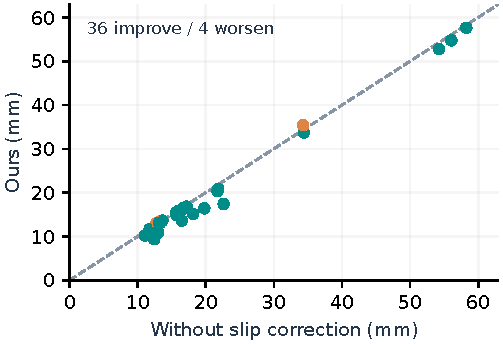
\includegraphics[width=\columnwidth]{figures/soft_scatter.pdf}
\caption{\textbf{Complete prospective SoftVT comparison.} Every dot is one of the 40 fresh episodes. All methods are scored on the same 1,998 forecast frames. Improvements mainly reflect placement and release rather than a change in internal deformation.}
\label{fig:soft}
\end{figure}

\paragraph{Forecast accuracy and coverage.}
Table~\ref{tab:soft} reports complete paired means. Slip-aware prediction improves the original mechanics/contact pipeline by 1.067\,mm (5.64\%) and improves the rigid/contact control by 3.66\%. It wins on 36 of 40 episodes against the original and 35 against the rigid/contact control. A descriptive paired episode bootstrap gives a 95\% interval of $[0.692,1.471]$\,mm for the mean improvement over the original. Since objects recur across episodes, this interval does not measure uncertainty over new object identities.

\begin{table}[h]
\centering\small\setlength{\tabcolsep}{3pt}
\caption{\textbf{SoftVTBench, 40 fresh episodes.} Lower is better; all methods listed have complete paired forecast coverage.}
\label{tab:soft}
\begin{tabular}{lr}\toprule
Method & Coordinate RMSE (mm)\\\midrule
Prefix-calibrated rigid & 20.002\\
Rigid with scene contact & 18.543\\
Mechanics with scene contact & 18.932\\
\textbf{Ours with slip/release} & \textbf{17.865}\\\bottomrule
\end{tabular}
\end{table}

\paragraph{What improved?}
Rigid-aligned shape error is 1.54517\,mm both before and after the slip correction. The gain therefore comes from predicting object motion and release, consistent with the mechanism of the update. This distinction matters: reducing world-coordinate error does not establish better elasticity identification. Across the full 220-case development and regression inventory, the robust predictor has complete trajectory coverage. Its numerical fallback repairs one inherited nonfinite trajectory; all 179 previously finite Phase A forecasts remain bitwise unchanged. The supplementary material separates that regression result from the fresh 40-episode table.

\subsection{PhysTwin: real sequence continuation}
We evaluate eight released plush-object sequences: single lift of sloth, dinosaur and zebra; single push of sloth; and double lift and double stretch of sloth and zebra. All eight were historically inspected, so this is an exploratory real-data evaluation. The adapter uses 240 mechanical nodes, 18 fitting frames from each observed prefix and at most 50 optimization iterations, with a fixed time budget. The recipe was chosen using development-prefix validation and then held fixed for the corrected-mask rerun.

The released motion-validity array describes transitions from $t$ to $t+1$. Our corrected position mask at time $t$ uses visibility at $t$ and the incoming validity at $t-1$; time zero uses visibility alone. This removes a one-frame look-ahead in the older adapter. Offline upstream tracking itself has not been certified causal. Primary real-data tables use only the corrected predictions; older exploratory results are identified separately in the supplement.

\paragraph{Geometry.}
Manual track error is the mean Euclidean distance per annotated point, averaged over valid forecast frames and then over sequences. All methods use initial-frame point matching. Displacement error subtracts each point's initial position before comparison. Pair-distance-change error measures changes in internal distances, removing rigid motion and reducing the influence of initial alignment offsets. It is a standard deformation diagnostic, not a new metric or a force measurement.

\begin{table}[h]
\centering\small\setlength{\tabcolsep}{3pt}
\caption{\textbf{Real PhysTwin, all eight sequences.} Track, displacement and pair-distance-change errors in mm. Every row completes its forecasts; lower is better.}
\label{tab:real}
\begin{tabular}{lrrr}\toprule
Method & Track & Displ. & Pair change\\\midrule
Position ridge & 29.04 & 28.90 & 18.85\\
Analytic adapter & 40.54 & 40.61 & 18.66\\
Ours, neural adapter & 39.01 & 38.90 & 16.96\\
\textbf{Released PhysTwin} & \textbf{21.14} & \textbf{21.04} & \textbf{10.52}\\\bottomrule
\end{tabular}
\end{table}

The neural law improves tracking by 3.76\% over the matched analytic adapter and reduces pair-distance-change error by 9.13\%. Native PhysTwin nevertheless remains substantially stronger on the complete within-sequence benchmark. Position ridge is also competitive in tracking, although its internal-distance error is larger than that of the neural adapter. These outcomes motivate treating motion, deformation and transfer as separate questions rather than using a single favorable score.

\paragraph{Shared-appearance image comparison.}
We evaluate three predetermined noninitial frames from each sequence in all three recorded cameras. Nine images per method per sequence are averaged equally. All trajectories use the same initial Gaussian appearance and local rigid transport. Crops derive from the reference foreground mask, with an eight-pixel margin; predicted spill inside this crop is retained. Table~\ref{tab:render} reports PSNR, SSIM, LPIPS and silhouette IoU under this common policy.

\begin{table}[h]
\centering\small\setlength{\tabcolsep}{3pt}
\caption{\textbf{Recorded-camera appearance, 72 images per method.} Shared initial Gaussians, fixed crops and no appearance refitting.}
\label{tab:render}
\begin{tabular}{lrrrr}\toprule
Method & PSNR$\uparrow$ & SSIM$\uparrow$ & LPIPS$\downarrow$ & IoU$\uparrow$\\\midrule
Analytic &16.04&.598&.329&.559\\
Ours &16.13&.599&.326&.561\\
\textbf{PhysTwin} &\textbf{17.66}&\textbf{.647}&\textbf{.264}&\textbf{.686}\\\bottomrule
\end{tabular}
\end{table}

\begin{figure*}[t]
\centering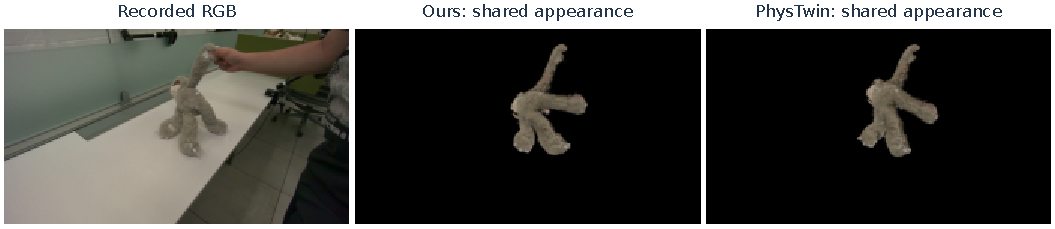
\includegraphics[width=\textwidth]{figures/render_comparison.pdf}
\caption{\textbf{A common appearance model exposes geometry differences.} Final frame of the first declared sequence, single-lift sloth, camera 2. Full images are shown. Rendered panels use identical initial Gaussian assets; the recorded RGB is a real observation.}
\label{fig:appearance}
\end{figure*}

PhysTwin's stronger trajectory prediction is accompanied by better image metrics. Ours does not achieve rendering parity on this cohort. Unrecorded-camera orbits remain useful qualitative inspections, but absent reference images they cannot demonstrate superior novel-view accuracy.

\subsection{PhysTwin: frozen cross-interaction transfer}
The transfer question differs from sequence continuation: can material fitted during one manipulation predict another interaction without fitting the new motion? We use five declared source--target pairs, transferring from single-lift sloth or single-lift zebra to pushing, two-hand lifting or stretching of the corresponding named object. Geometry is rigidly registered using only the target initial configuration. All later target object observations are withheld from adaptation.

\paragraph{Initial-geometry compatibility.}
A fixed gate requires symmetric median registration distance below 3\% and 95th-percentile distance below 8\% of the source bounding-box diagonal. It uses no future target motion. Two pairs pass: sloth lift to push, and zebra single-hand to two-hand lift. Three stretching/lifting pairs fail and remain diagnostic results. The gate tests geometric compatibility, not independently verified semantic correspondence or a guarantee that initial material states are identical.



\paragraph{Frozen adaptation protocol.}
Our source material field and constitutive weights remain fixed. New attachment locations follow target initial geometry and known tools, with median source attachment strength. The native comparator retains its fitted object springs and uses new geometric controller springs with median source stiffness. Both methods receive the same source-to-target registration. A persistent registered source shape gives a simple no-response control. Matching to manual target tracks uses the same initial canonical source points for all methods.

We score every noninitial frame of the target interaction, not only its official forecast suffix. These results therefore measure source-to-new-interaction transfer and should not be numerically compared to Table~\ref{tab:real}, which scores continuation suffixes. Training budgets and physical parameterizations differ between the released native model and our adapter; the comparison measures the resulting configured pipelines.

\begin{table}[h]
\centering\small\setlength{\tabcolsep}{3pt}
\caption{\textbf{Two qualifying real interaction pairs.} Equal-pair mean over the full noninitial target interaction. All methods complete both trajectories. Errors are in mm.}
\label{tab:transfer}
\begin{tabular}{lrrr}\toprule
Method & Track & Displ. & Pair change\\\midrule
Source-shape persistence &79.11&70.79&17.25\\
Frozen PhysTwin adaptation &44.63&34.97&16.85\\
Analytic adapter &40.90&29.60&16.71\\
\textbf{Ours, neural adapter} &\textbf{39.16}&\textbf{27.34}&\textbf{16.20}\\\bottomrule
\end{tabular}
\end{table}

\paragraph{Results.}
The neural adapter reduces mean tracking error by 12.26\% and displacement error by 21.81\% relative to the frozen native adaptation. The pair-distance-change improvement is smaller, 3.82\%. Thus the largest benefit concerns changed motion under the new interaction, while internal deformation remains difficult. Compared with the analytic adapter, the neural law improves tracking by 4.26\%, a modest but consistent aggregate contribution beyond the analytic response family.

Both qualifying pairs and all five diagnostic pairs are listed in the supplement. The ungated five-pair diagnostic mean is 34.29\,mm for ours and 46.02\,mm for the frozen native adaptation. We do not promote that more favorable percentage to the primary transfer claim because three initial geometries fail the declared compatibility test. The two-pair pilot supports further transfer evaluation, not a population-level claim of real-world OOD superiority.

\section{Analysis and Discussion}
\begin{figure}[h]
\centering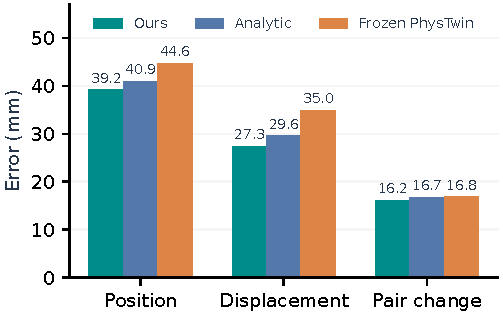
\includegraphics[width=\columnwidth]{figures/transfer_compact.pdf}
\caption{\textbf{Decomposing the real-transfer gain.} World position, displacement from the initial state, and internal distance changes are distinct observables. The largest gap is in motion; the internal-deformation advantage is smaller. Each bar averages the same two qualifying pairs.}
\label{fig:metrics}
\end{figure}

\paragraph{Which part of the model helps?}
The SoftVT ablation isolates the added slip-release rule: its original shape predictions remain essentially unchanged, yet placement improves. This is evidence for modeling the interaction state rather than attributing all motion to elasticity. The PhysTwin analytic-versus-neural comparison instead holds the external geometry and equilibrium interface fixed while changing the bulk response. Its smaller improvement indicates that a reusable constitutive prior is helpful, but does not remove errors caused by initialization, contacts, geometry or the quasistatic approximation.

These findings also clarify why a purely position-based regression control can be strong. When test commands resemble the observed prefix, interpolation in control space can predict motion well without recovering mechanics. Such a control is essential for interpreting a twin's gains. It does not, however, provide independent evidence about forces or guarantee transfer to another interaction. We retain it in the complete continuation table rather than omitting it in favor of weaker controls.

\paragraph{Numerical sanity and physical accuracy.}
A positive tetrahedral determinant checks local validity of the chosen discrete deformation. Finite trajectories and complete frame coverage check availability. Contact penetration and residual norms can reveal numerical failures. None of these quantities is itself a measured force or proof that the material law matches the real object. Our equilibrium anchor enforces a Jacobian cutoff, but empirical output corrections and reduced pose/contact operations are separate stages; an anchor's validity cannot automatically be assigned to all adapted outputs.

Likewise, photometric agreement measures the rendered observation under a particular camera and appearance model. It can improve because of geometry, texture, opacity, visibility or transport. By freezing the initial appearance and using common crops, we isolate some of these factors, but we do not convert PSNR into a physical calibration score. Real force accuracy would require independent measurements or additional controlled physical observations.

\paragraph{Limits of the current representation.}
Initial geometry and correspondences are provided. Unknown prestress, density and reconstruction errors can be absorbed into effective scene parameters. SoftVT contact is a split rigid-pose approximation, while the real adapter uses quasistatic equilibrium with explicit attachments and floor support. Neither benchmark establishes a general coupled model of arbitrary rigid and deformable objects, frictional sliding, impact or changing topology. The learned law covers a restricted elastic family rather than plasticity or material history. Calibrated uncertainty and an uncertainty-driven action policy are not claimed.

\paragraph{Reproducibility.}
The accompanying source package contains the manuscript, generated figures, exact metric sources, per-case tables and figure-selection rules. Numerical results are taken from frozen saved evaluations; no model is retuned for this paper. The supplementary protocol distinguishes the corrected real-data results from earlier exploratory configurations and preserves their stronger historical scores without mixing them into the current comparison. Data, checkpoints and prediction arrays remain external assets with provenance recorded in the development archive.

\section{Conclusion}
Position-driven twins benefit from separating what moves with material, what is defined relative to a tool, and what acts in the world. A reduced slip-release model improves complete SoftVT forecasts, and a frozen constitutive adapter yields promising transfer across two real interactions. The full real-data evaluation also shows where a native spring-mass twin remains stronger. Evaluating placement, deformation and rendering separately makes these results interpretable and provides a concrete basis for improving physical prediction beyond matching observed motion.

\clearpage
\section*{LLM Usage Statement}
OpenAI Codex assisted with implementation, experiment orchestration, literature discovery, result checks, manuscript drafting and programmatic figure generation. This manuscript consolidates saved experiments; figures are generated from their artifacts rather than synthesized as experimental evidence. The authors are responsible for validating all methods, results, references and the final submission.
{\small\bibliographystyle{ieeenat_fullname}\bibliography{references}}
\end{document}
